\subsection{Exponential Decay}\label{ex:decay-set-sample}

set-based and sample-based, two data points but show two possible choices.
invert the correct set but do make note that in order to do so, we needed to have observed a perfect signal, which is unrealistic.


\begin{figure}[h]
\begin{minipage}{.475\textwidth}
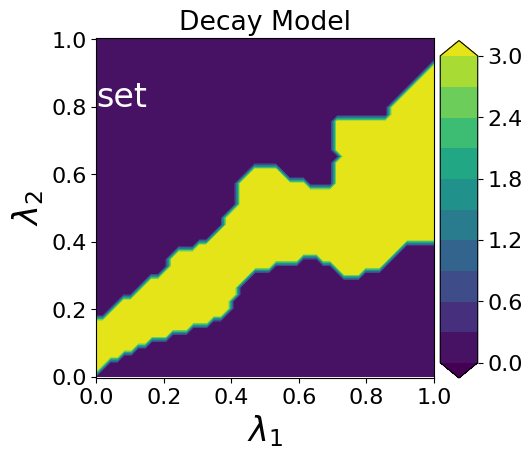
\includegraphics[width=\linewidth]{examples/fig_decay_q1/DecayModel--set_N50_em.png}
\end{minipage}
\begin{minipage}{.475\textwidth}
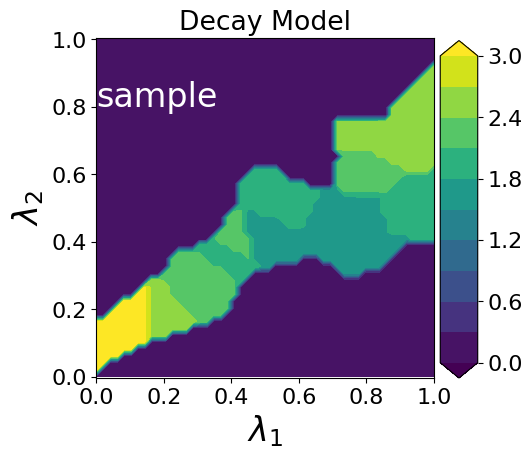
\includegraphics[width=\linewidth]{examples/fig_decay_q1/DecayModel--sample_N50_mc.png}
\end{minipage}
\caption{The inverse image of the reference measure for set-based (left) and sample-based (right) solutions for $N=50$ parameter samples.}
\label{fig:heatrod-sol-ex}
\end{figure}
